%Planejamento da Escrita. Desktop do pesquisador: ferramentas. Perfis científicos. Mapeamento Sistemático

\section{Textos acadêmicos como projetos}

%%
\begin{frame}{Gestão e planejamento}
\begin{itemize}
\item Produzir artigos, dissertações ou teses depende de planejamento
\item Tempo médio para escrever sua pesquisa: 3 - 6 meses (empirismo) 
\item Cada texto é um projeto: planejamento, execução, entrega
\item Um bom texto é fruto de um bom planejamento
\end{itemize}
\end{frame}

\subsection*{Ferramentas para gestão de projetos}

%%
\begin{frame}{Métodos e ferramentas}
\begin{itemize}
\item \textit{Getting Things Done}: \url{http://gettingthingsdone.com}
\item Trello: \url{http://trello.com}
\item MS Project, Asana, Google Sheets + Gantt, etc.
\item Slack (+ orientador e colaboradores) \\
>> O importante é você encontrar a sua forma de organização!
\end{itemize}
\end{frame}

%%
\begin{frame}{Outros métodos}
Você poderá adaptá-los:
\begin{itemize}
\item Scrum/Sprint
\item Kanban
\item PMBOK
\item PDCA
\end{itemize}
\end{frame}

\section{Ferramentas para anotações}

%%
\begin{frame}{Ferramentas para anotações}
\begin{itemize}
\item Evernote (minha preferência)
\item Google Keep, Soho Notes, Google Docs
\item MS Onenote, Apple Notes
\end{itemize}
\end{frame}

%%
\begin{frame}{Exemplo}
\begin{figure}
\centering
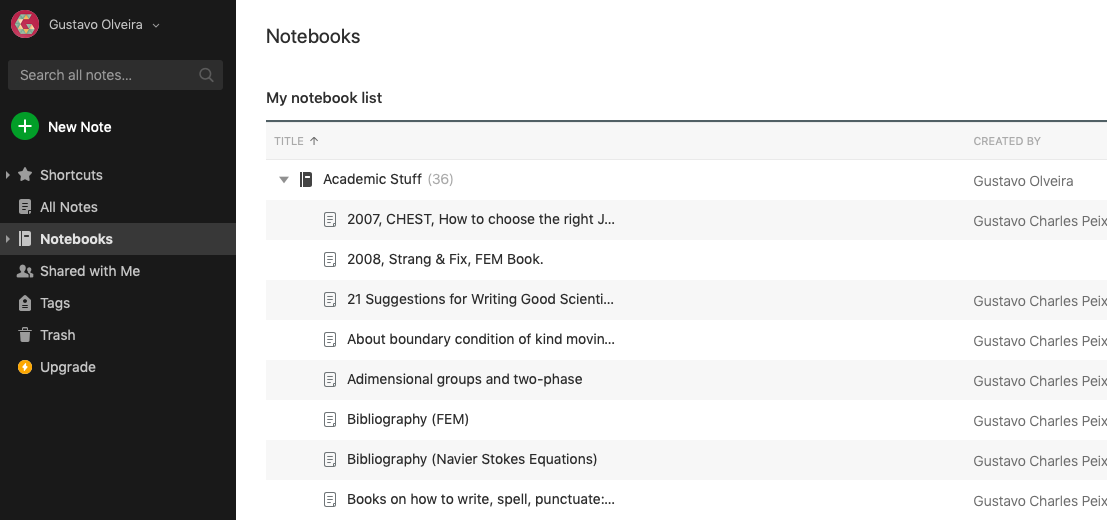
\includegraphics[scale=0.3]{figs/02/evernote}
\caption{Notebooks acadêmicos do Evernote. Fonte: Arquivo pessoal.}
\end{figure}
\end{frame}

%% 
\begin{frame}{O poder das anotações}
\begin{itemize}
\item \textit{Note-making} é uma forma eficiente de organizar idéias
\item Fundamental em aulas e na leitura de bibliografias gerais
\item Ajudam a encontrar o essencial
\item Impedem que você não seja engolido pela literatura
\end{itemize}
\end{frame}

%%
\begin{frame}{Modelos de \textit{note-making}}
Ajudarão você a:
\begin{itemize}
\item construir notas em um formato claro e legível 
\item lembrar-se do tipo de informação que você deseja registrar em cada fonte
\item padronizar suas notas de modo a encontrar particularidades mais facilmente
\end{itemize}
\end{frame}

%%
\begin{frame}{O que o modelo contempla?}
\begin{enumerate}
\item Registro de todos os detalhes da referência
\item Esqueleto baseado em cabeçalhos (folha de conceito)
\end{enumerate}
\end{frame}

%%
\begin{frame}{Exemplos de cabeçalhos}
\begin{itemize}
\item principal propósito do texto
\item principais evidências
\item principais argumentos
\item métodos usados
\item principais descobertas
\item pesquisas futuras
\end{itemize}
\scriptsize{Veja: \url{https://www2.le.ac.uk/offices/ld/resources/study/notes}}
\end{frame}

%%
\begin{frame}{Exemplo}
\begin{figure}
\centering
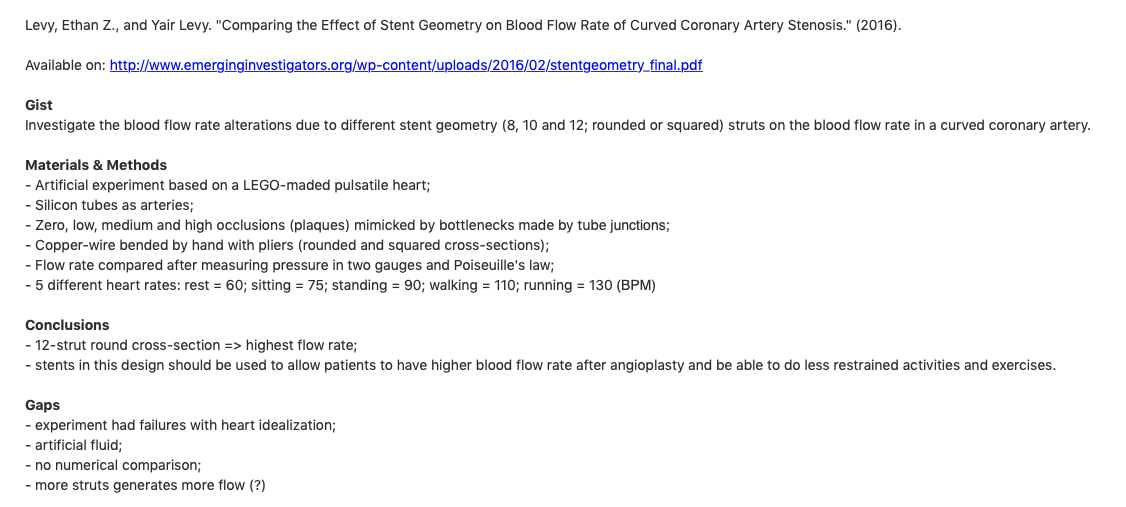
\includegraphics[scale=0.3]{figs/02/note-making}
\caption{Note-making de artigo. Fonte: Arquivo pessoal.}
\end{figure}
\end{frame}

%%
\begin{frame}{Diário de bordo}
\begin{itemize}
\item Conte sua história durante a pós
\item Mantenha um diário para registrar conquistas, tristezas, avanços, retrocessos
\item Registre parâmetros usados em experimentos, modelos, etc. 
\end{itemize}
\scriptsize{Veja: \url{http://www.e-diariodebordo.com.br}}
\end{frame}

%%
\begin{frame}{Exemplo}
\begin{figure}
\centering
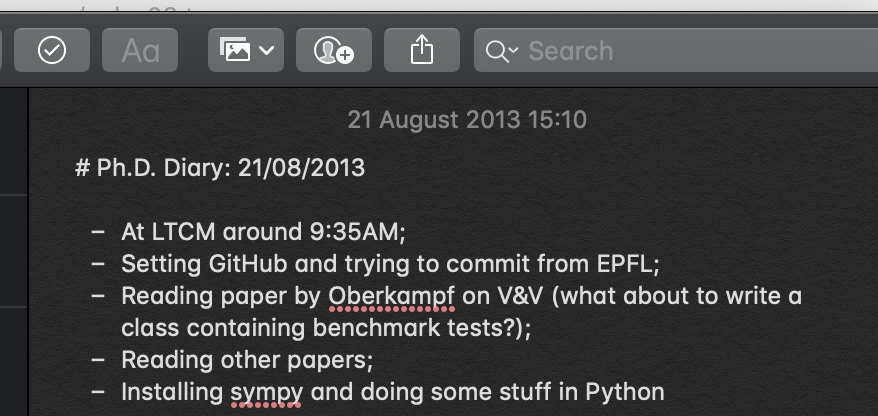
\includegraphics[scale=0.5]{figs/02/diario}
\caption{Fragmento de diário do Ph.D. Fonte: Arquivo pessoal.}
\end{figure}
\end{frame}

\section{Ferramentas para desenho, diagrama e canvas}

%%
\begin{frame}{Mapas mentais/mapas de conceito}
Mapas mentais (\textit{mind maps}) ajudam a ter visão global de um assunto.
\begin{itemize}
\item Mindmap Maker
\item Google Drive + MindMup
\item Freemind
\item Coggle
\end{itemize}

Procure também por: \texttt{concept sheet}.
\end{frame}


%%
\begin{frame}{Fluxogramas e diagramas}
\begin{itemize}
\item OmniGraffle 
\item Lucidchart
\item draw.io (recomendado)
\end{itemize}
\end{frame}

%%
\begin{frame}{Canvas simples e avançado}
\begin{itemize}
\item canvas.com (recomendado)
\item CorelDraw
\item Inkscape (recomendado)
\item Adobe Illustrator
\end{itemize}
\end{frame}

\section{Ferramentas para gerenciamento bibliográfico}

%%
\begin{frame}{Ferramentas para gerenciamento bibliográfico}
\begin{itemize}
\item Mendeley (recomendado)
\item Readcube
\item Endnote
\item Zotero
\item Bibdesk, Jabref (veremos em aulas posteriores)
\end{itemize}
\end{frame}

%%
\begin{frame}{Exemplo}
\begin{figure}
\centering
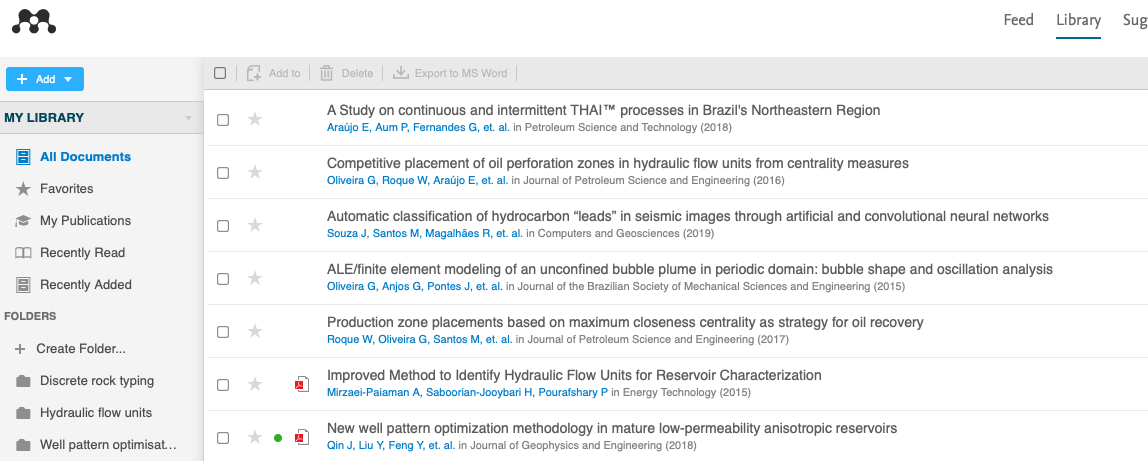
\includegraphics[scale=0.25]{figs/02/mendeley}
\caption{Biblioteca do Mendeley. Fonte: Arquivo pessoal.}
\end{figure}
\end{frame}

%%
\begin{frame}{Exemplo}
\begin{figure}
\centering
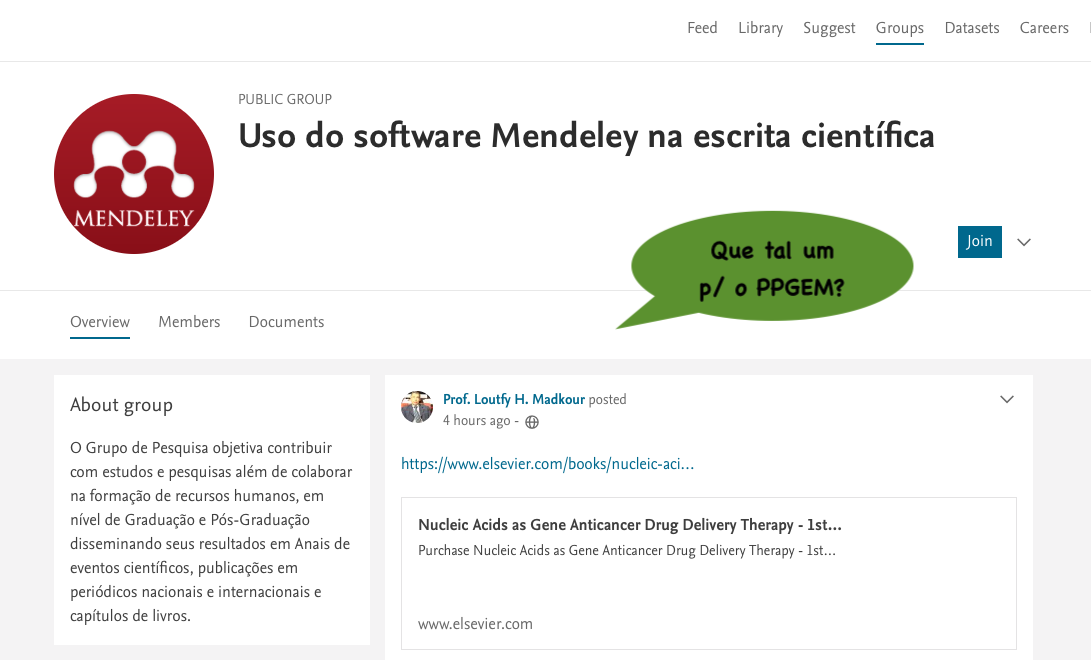
\includegraphics[scale=0.25]{figs/02/mendeley-ppgem}
\caption{Grupo do Mendeley. Fonte: site Mendely.}

\scriptsize{Veja: https://bit.ly/2OGY0PR}
\end{figure}
\end{frame}


\section{Perfis científicos}

%%
\begin{frame}{Identificadores digitais}
\begin{itemize}
\item Carteira de identidade do autor (código digital)
\item Existem vários sistemas de identificação: Scopus ID, Researcher ID, Lattes ID, Google ID, etc.
\item Registro central de identificadores de autores: \textbf{ORCID}
\end{itemize}
\end{frame}


%%
\begin{frame}{ORCID: \textit{Open Researcher and Contributor ID}}
\begin{itemize}
\item Integra todos os outros identificadores
\item Proporciona visibilidade internacional 
\item Integrador de dados
\item Registra suas publicações em um único local
\item Resolve problemas de ambiguidade de homônimos
\item Cria uma ``rede social'' de pesquisadores da mesma área
\end{itemize}
\end{frame}

%%
\begin{frame}{Como obter o seu ORCID?}
\begin{figure}
\centering

\includegraphics[scale=0.6]{figs/02/orcid}
\end{figure}

Cadastre-se em \url{http://orcid.org}

\scriptsize{Veja: \url{https://bit.ly/2S31wjU}}

\end{frame}

%%
\begin{frame}{ResearchGate}
\begin{figure}
\centering

\includegraphics[scale=0.4]{figs/02/rg}
\end{figure}
\begin{itemize}
\item A ``rede social'' dos pesquisadores
\item Compartilhamento de publicações e projetos
\item Q{\&}A
\item Ofertas de trabalho
\end{itemize}

\scriptsize{Veja: \url{https://bit.ly/2yILdl1}}
\end{frame}

%%
\begin{frame}{CV Lattes}
A porta de entrada...

\begin{figure}
\centering

\includegraphics[scale=0.4]{figs/02/cvlattes}
\end{figure}
\begin{itemize}
\item Se não criou, crie!
\item Mantenha-o atualizado!
\end{itemize}

Veja: \url{https://lattes.cnpq.br}
\end{frame}

%%
\begin{frame}{coneCTIbrasil}
\begin{figure}
\centering

\includegraphics[scale=0.3]{figs/02/conecti}
\end{figure}
\begin{itemize}
\item Proposta de integração de informações
\item Adoção de identificadores persistentes: ORCID, DOI, ISBN e ISSN
\item Interoperabilidade dos PPGs nacionais e produções
\item Pesquisadores preencherão informações em único local
\end{itemize}
Veja: \url{https://www.conectibrasil.org}
\end{frame}

\section{Mapeamento e revisão sistemáticos}

%%
\begin{frame}{Pesquisa secundária}
\begin{itemize}
\item Estudos primários são originais; inéditos
\item Estudos secundários procuram tirar conclusões a partir dos primários;
\item ESs integram e sintetizam as descobertas 
\item Objetivo principal: \textbf{identificar lacunas de pesquisa}
\end{itemize}
\end{frame}

%%
\begin{frame}{Mapeamento sistemático (MS)}
\begin{block}{O que é?}
Uma revisão ampla dos estudos primários existentes em um tópico de pesquisa para identificr se há subtópicos nos quais mais estudos primários são necessários.
\end{block}
\begin{itemize}
\item MSs identificam clusters de estudo e visam apenas classificar a literatura relevante 
\item Focam-se na estruturação de uma área de pesquisa
\item Análises são em escopo amplo
\end{itemize}
\end{frame}

%%
\begin{frame}{Revisão sistemática (RS)}
\begin{block}{O que é?}
Uma revisão dos estudos primários em termos de seus resultados que investiga se estes são consistentes ou contraditórios.
\end{block}
\begin{itemize}
\item RSs são mais detalhadas e agrega resultados relacionados a uma questão de pesquisa específica
\item RSs envolvem menos trabalhos e mais profundidade.
\item Análises são em escopo restrito
\end{itemize}
\end{frame}

%%
\begin{frame}{MSs e RSs são abordagens complementares}
Razões para realizar MSs:
\begin{itemize}
\item Examinar a extensão e a natureza de uma atividade de pesquisa
\item Avaliar o valor do esforço e necessidade de se realizar uma RS completa
\item Coletar e resumir a pesquisa existente em um tópico (fundamental para doutorandos em início de trabalho)
\item Identificar lacunas existentes que apontem para subtópicos promissores
\end{itemize}
\end{frame}

%%
\begin{frame}{MSs e RSs são abordagens complementares}
Razões para realizar um MS antes da RS:
\begin{itemize}
\item Reduzir o tempo restante com pesquisa subsequente
\item Facilitar a compreensão da literatura e definição das questões de pesquisa
\item Rastrear tendências de pesquisa
\item Aprender mais sobre o tópico estudado
\end{itemize}
\end{frame}

%%
\begin{frame}{Desafios}
\begin{itemize}
\item MS pode consumir muito tempo
\item No doutorado, um MS pode se estender além do estipulado, mas sendo de qualidade, publicações são quase garantidas
\item Para mestrado, é importante avaliar o tópico com cuidado, pois um MS completo pode ser inviável.
\item A seleção e classificação depende de experiência
\item Orientadores servem para guiarem você à familiarização com a nova terminologia
\end{itemize}
\end{frame}

%%
\begin{frame}{O processo}
\begin{figure}
\centering
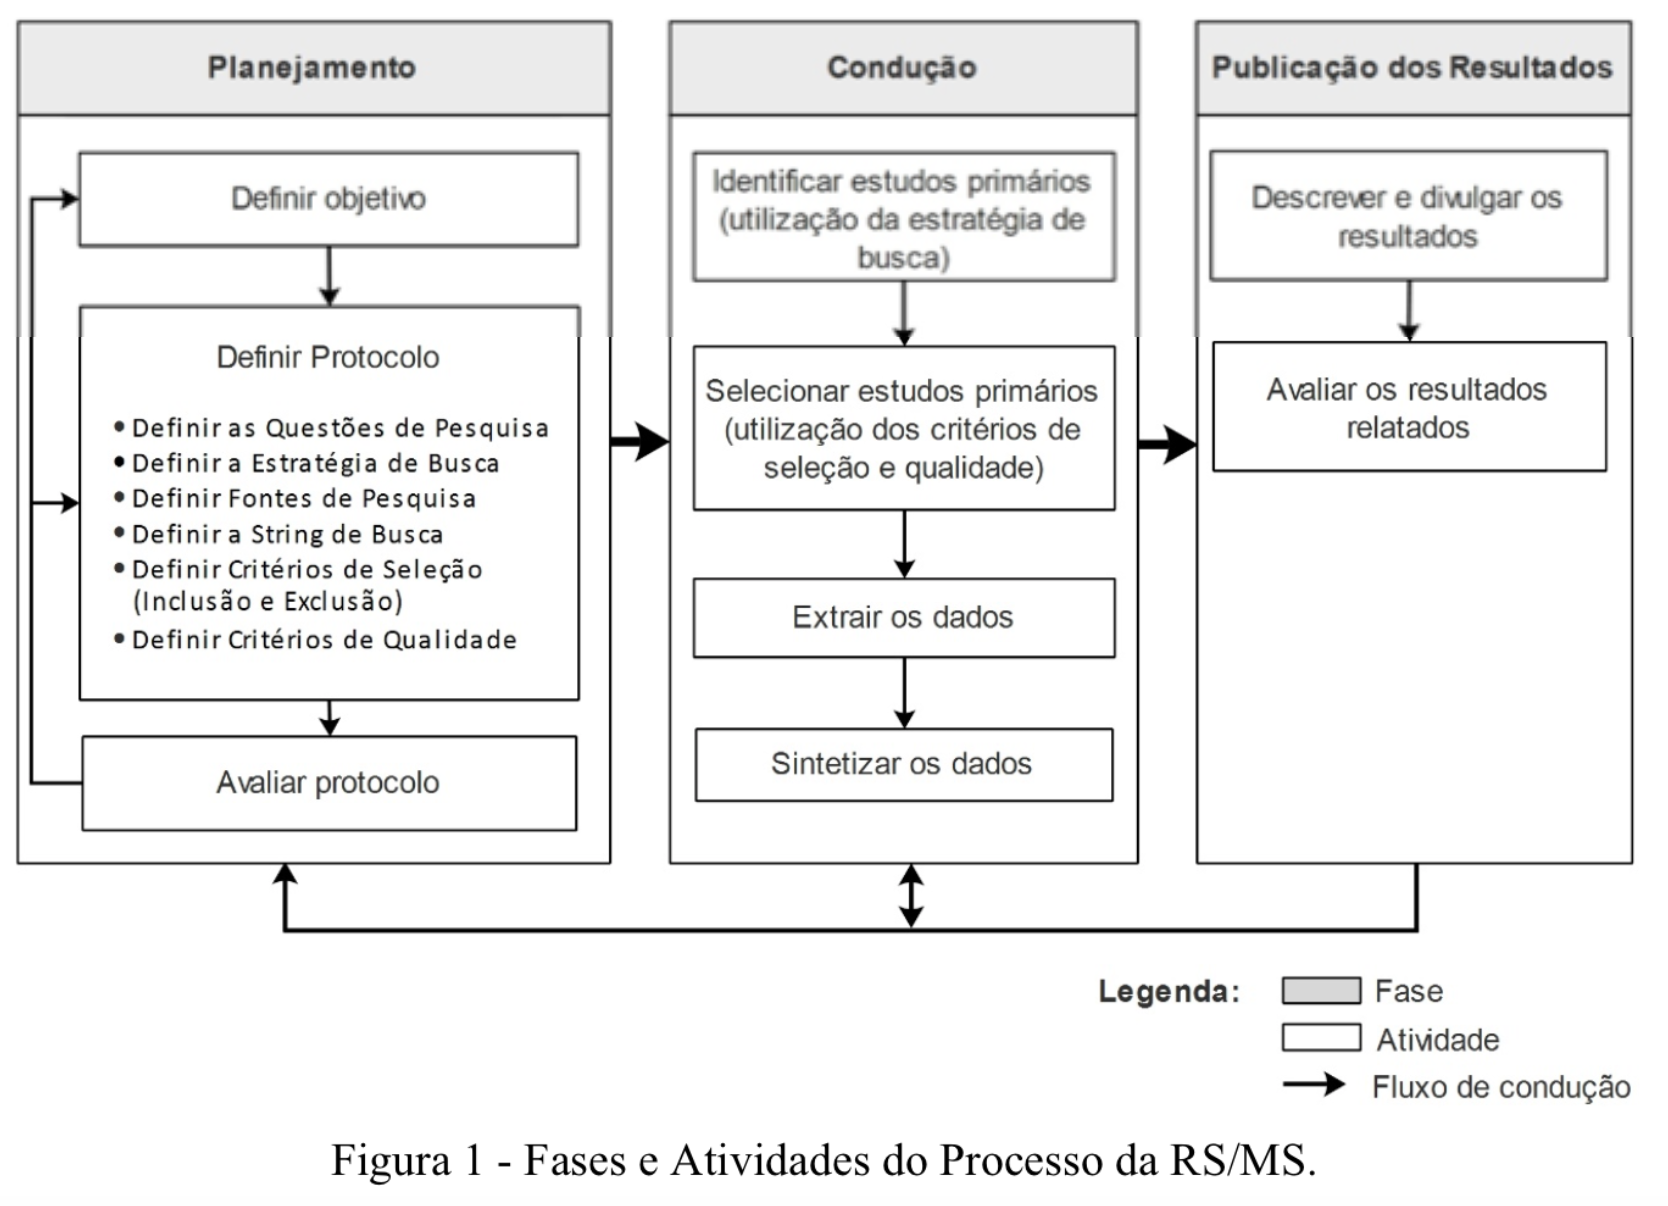
\includegraphics[scale=0.3]{figs/02/ms}
\caption{Processo do MS. Fonte: Salbo, 2018.}
\end{figure}
\end{frame}

%%
\begin{frame}{Ferramentas para MS}
\begin{itemize}
\item Existem várias ferramentas para MS
\item CADIMA, ReLiS, Parsifal
\item Veja o espaço SR Toolbox: \url{http://systematicreviewtools.com/index.php}
\item Veja este artigo: \url{https://bit.ly/2Tnj9gM}
\item Veja o projeto: \url{http://nailsproject.net}
\end{itemize}
\end{frame}

%%
\begin{frame}{Exemplo: Parsifal}
Parsifal é uma excelente ferramenta para MS: \url{https://parsif.al}.
\begin{figure}
\centering
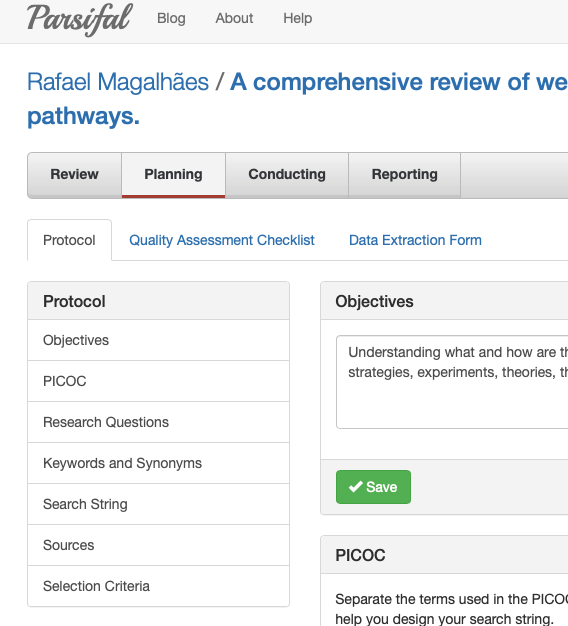
\includegraphics[scale=0.2]{figs/02/ms2}
\caption{Parsifal. Fonte: Autor.}
\end{figure}
Veja: \url{https://bit.ly/2MNCmH3}
\end{frame}


\subsection{MS com Parsifal: hands-on}

%%
\begin{frame}{Criando um MS fictício}
\begin{block}{Revisão}
\begin{itemize}
\item Título: Impactos do ensino da escrita científica no desenvolvimento de pós-graduandos
\item Descrição: Mapeamento sistemático sobre os impactos do ensino da escrita científica no primeiro período da pós-graduação sobre a produção acadêmica dos estudantes do programa.
\end{itemize}
\end{block}
\end{frame}

%%
\begin{frame}
\begin{block}{Planejamento}
\begin{itemize}
\item Objetivo: Buscar uma ementa eficiente para a disciplina
\item PICOC: P - mestrandos, doutorandos; I - consulta pública; enquete; O: didática; engajamento
\end{itemize}
\end{block}
\end{frame}

%%
\begin{frame}
\begin{block}{Planejamento: questões de pesquisa}
\begin{itemize}
\item Mapeamento sistemático é um tópico relevante para a disciplina 'Produção Científica'?
\item O conceito de mapeamento sistemático será melhor absorvido pela classe se o professor incluir exemplos práticos?
\item A satisfação do estudante em relação à ementa é um parâmetro considerável para reformulá-la?
\end{itemize}
\end{block}
\end{frame}

%%
\begin{frame}
\begin{block}{Planejamento: keywords}
\begin{itemize}
\item aluno de mestrado; mestrando
\item aluno de doutorado; doutorando
\end{itemize}
\end{block}

\begin{block}{Planejamento: string de busca}
\texttt{("aluno de doutorado" OR "doutorando" OR "aluno de mestrado" OR "mestrando" OR "aluno especial")|}
\end{block}

\begin{block}{Planejamento: fontes}
\begin{itemize}
\item Web of Science
\item Scopus
\end{itemize}
\end{block}
\end{frame}

%%
\begin{frame}
\begin{block}{Condução}
\begin{itemize}
\item Importar artigo: `de2017stress'
\item Classificar como aceito
\item Avaliar qualidade
\end{itemize}
\end{block}

\begin{block}{Condução}
\begin{itemize}
\item Extrair dados
\item Análise de dados
\end{itemize}
\end{block}

\begin{block}{Resumo}
\begin{itemize}
\item Gerar relatório
\end{itemize}
\end{block}
\end{frame}

%%
\begin{frame}{Desafio em grupo}
\begin{itemize}
\item Grupos de 5 alunos em área de pesquisa comum
\item Construir MS com no mínimo 20 artigos (4 por aluno)
\item Tema de pesquisa: interesse do grupo
\item Gerar questões de pesquisa e um MS sobre o assunto
\end{itemize}
\end{frame}


%%{}

\begin{frame}{Sugestão de leitura...}

\url{http://betterthesis.dk} 

\url{https://finishyourthesis.com/write-literature-review/}

\end{frame}

%% === REFS
\begin{frame}[allowframebreaks]
\frametitle{Referências}
\begin{thebibliography}{9}
\setbeamertemplate{bibliography item}[book]
%
\bibitem{falbo2018}Falbo, R. A. \textit{Mapeamento Sistemático}. UFES, Outubro, 2018.
%
\bibitem{cooper1998}Cooper, H. \textit{Synthesizing research: A guide for literature reviews}. Sage, 1998.
%
\bibitem{charters2007}Kitchenham, B.A., Charters, S. \textit{Guidelines for performing systematic literature reviews in  software engineering}, Keele University, 2007.
%
\bibitem{petersen2008}Petersen, K. et al. \textit{Systematic mapping studies in software engineering}, Ease, 2008.

\bibitem{kohl2018}Kohl, Christian, E. J. et al. \textit{Online tools supporting the conduct and reporting of systematic reviews and systematic maps: a case study on CADIMA and review of existing tools}, \textit{Environmental Evidence} 7(1), 2018.

\end{thebibliography}
\end{frame}